\chapter{Hardware Design and Implementation}


\section{Mechanical Hardware}
\subsection{Mechanical Components}
\subsection{Motor}
\subsection{Assembly}



\section{Electronic Hardware}
\subsection{System Description}

% Show block diagram of the system and explain the functioning og the system
\begin{figure}[h]
	\centering
	\input{"./figs/Electronic_System/ElectronicSystemOverview.tikz"}
	\caption{Electronic System Overview}
	\label{fig:electronicSystemOverview}
\end{figure}



Figure \ref{fig:electronicSystemOverview} provides a system overview and how the different parts functions together. The micro-controller receives the different signals that has been correctly conditioned from supporting circuitry to interpret the dynamics of the system. From the observed condition it is able to output the correct signals to instruct the next command.

The digital logic circuit that consist of logic level converters acquires the signal from the micro-controller and performs signal conditioning to interface with the motor driver and determines the correct direction to rotate the motor. 

The motor driver controls the DC brushed motor based of the digital signals and provides a proportional feedback current that is delivered to unity-gain amplifier.

The motor contains a encoder that indicates the direction and position of the rotor through digital signals that is sent through a digital logic filter to retrieve only critical information from the encoder signals. 

The physical model contains a potentiometer that measures the non-actuated pendulums angle and is sent to the buffer.

The microcontroller will use the UART interface as it's data acquisition protocol to send the necessary information to the computer. 

The micro-controller is programmed using the Serial Wire Debug (SWD) protocol to transfer the binaries from the computer.

Power is provided using a external 12V power-supply, which will power the motor, but also using a regulator to down convert/step to a 5V and 3.3V to power the microcontoller and the other peripherals.


\subsection{Microcontroller}
The microcontroller chosen is the STM32F030Mxx. The selection was done according the ease of setting up, memory size, physical dimensions and the peripherals it provided.

The STM32F030MXX is based of the ARM M0 architecture which is ARM's entry level micro-controller. It requires little support to have a up and running microcontroller requiring only the SWD protocol to program and a few by-pass capacitors.

It was difficult to determine the memory size specification for the project. This uncertainty ensured that the largest memory size the ARM M0 architecture could provide was selected.

The Electrical and Electronic Department's Printed Circuit Board (PCB) manufacturing machine can only provide a  minimum track width \SI{0.3}{mm}. This resulted in choosing a microcontroller whose footprint would meet the requirement.

Based on the conceptual design, the chosen microcontroller required to contain 2 ADC's, minimum of 5 GPIO's and 1 serial communication peripheral.

\subsubsection{Programming / Debug Interface}
The \textit{Atollic TrueSTUDIO for ARM 8.0.0} Integrated Development Environment (IDE) is used for writing the source code which converts the source code to the Executable and Linkable Format (.elf) file. These .elf files is then written using the Serial Wire Debug (SWD) protocol to the $\mu$C. Debugging of the source code occur using the same IDE which allows the programmer to inspect variables, timers and logic.

\subsubsection{PC UART Interface }

The purpose of the UART to serial communication is for data acquisition of the system response and for debugging purposes. The data being sent follows a structure to ensure the reliability of the data. Figure (ref) shows the format of the data being sent.

The data being sent across the UART to serial circuit is retrieved by a computer executing a Python script, listening for any activity on the computer's driver ports and writing the data into a comma-separated value (csv) file that can later be use to analyse the data.


The UART to serial circuit has been tested by doing a loopback test and using a digital logic analyser to verify the data being sent. The loopback test consist of connecting the Tx and Rx lines together and forcefully echo what has been sent to the circuit to be sent back. Figure (ref) in Appendix XXX shows the digital signals sent and received and confirms the working of the UART to Serial circuit. 

\subsection{Voltage Regulation}

The various components required different supply voltages in the electronic design. The diffenrent supply voltage is tabulated in table \ref{table:supplyVoltage}.

\begin{table}[]
	\centering
	\begin{tabular}{|c|c|}
		\hline
		Component & Supply Voltage [\SI{}{V}] \\
		\hline
		\hline
		Digital Logic Components & \SI{5}{} \\
		\hline
		$\mu$Controller & \SI{3.3}{} \\
		\hline
		Motor Driver & \SI{12}{} \\
		\hline
	\end{tabular}
	\caption{Suppy Voltage's for the different components}
	\label{table:supplyVoltage}
\end{table}


The table indicates 3 different supply voltages that will be required: \SI{3.3}{V}, \SI{5}{V} and \SI{12}{V}. This was achieved by using a \SI{5}{V} and \SI{3.3}{V} linear voltage regulators and the \SI{12}{V} is supply by a external source.

The schematic for each voltage regulator is shown in Appendix XX, where each voltage regulator circuit includes a Light Emitting Diode (LED) to ensure the minimum load is met for each regulator. The LED also acts as a visual debugging method.

\subsection{Potentiometer Sensor}
\subsubsection{Working Principle}
\begin{figure}[h]
	\centering
	\input{"figs/potentiometer/potentiometer.tikz"}
	\caption{Simplified Model of a Potentiometer}
	\label{fig:potentiometer}
\end{figure}
The rotary position potentiometer consist out of a wiper that is attached to a rotating shaft. The wiper relative position to a internal resistor is proportionally changed with rotation. The position of the wiper will output a voltage signal that is proportional to the position of the wiper relative to the resistor. 

\subsubsection{Interface}
The signal produced by the rotary potentiometer varies from 4.95V and 50mV from 360\textdegree to 0\textdegree respectively. This is signal sent through a simple voltage divider circuit to reduce the signal to 3V to 15mV to be within the sampling limits of the micro-controller. The reduce signal is then sent through a rail-to-rail unity gain amplifier before being sampled by the ADC of the microcontroller.

The scaled voltage is sent through a unity gain rail-to-rail amplifier, where the mirrored output signal is fed into the ADC. The type of ADC used in the STM32F030XX is a successive approximation register (SAR), \citep{stm32_ADC:2017}. The SAR ADC's contains internal capacitors that suffers from the effect of being depleted if the sampling frequency is to high. Using an operational amplifier reduces the risk of depleting this internal capacitor because of the low output resistance.

\begin{figure}[h]
	\centering
	\input{"./figs/unitygain/unitygain.tikz"}
	\caption{Unity Gain Amplifier Circuit}
	\label{fig:unitygain}
\end{figure}


\subsection{Magnetic Encoder}
\subsubsection{Working Principle}
A rotating gear containing ferrous metal teeth is attach to the rotating shaft. The rotating metal teeth rotates near a hall-effect sensor which creates a change in the magnetic flux inside the hall-sensor. This change in magnetic flux is sensed by the hallsensor which produces a digital signal \citep{hallsensor}.
\subsubsection{Digital Interface} 

\begin{figure}[h]
	\centering
	\input{"figs/JK_XOR_gates/jk_xor_nor.tikz"}
	\caption{Digital Logic Circuit containing JK-Flipflops, XOR- and NOR Gates}
	\label{fig:jk_xor}
\end{figure}

The encoder contains a sold state hallsensor which provides 2 channels with a 90 degree phase difference \citep{faulhaberencoder}. These 2 signals under go a hardware filter that produces 2 signals that indicate the direction of the motor and the incremental position.\\

The hardware filter consist out of XOR, NOR and JK-Flipflop gates shown in Figure \ref{fig:jk_xor} and the schematic in Figure \ref{sch:jk_xor}. The XOR gate produces the incremental position of the motor whereas the NOR and JK-Flipflop combination produces the direction of the motor by a logical 1 or 0.



The hardware filter was implemented to reduce the processing time of the micro-controller on the original signals.



%% Explain the effect of the gates maybe produce a signal table




These signals will be read by the $\mu$C using interrupts when a rising- \& falling edge are present.

The encoder provides 16 lines per revolution, equal to a combined 32 rising- \& falling edges per line. The encoder provides 2 lines increasing the resolution to 64. The motor is connected to a gearbox with a reduction stage of 14:1. The encoder will thus rotate 14 times per shaft revolution, increasing the resolution to 896 per revolution.

\subsection{Motor Driver}
\begin{figure}[h]
	\centering
	\input{"./figs/feedback_current/feedback_current.tikz"}
	\caption{Simplified Circuit of Motor Feedback}
	\label{fig:feedback_current}
\end{figure}

The motor driver IC is connected directly to the motor and responsible for directional and rotational control of the brushed DC motor. The motor driver is the MC33887 and contains 2 half H-bridges that forms a full H-bridge which are Pulse-Width-Modulated (PWM) to control the speed of the motor. The PWM- and direction signal originates from the micro-controller. As discussed previously, the signals' logic level is first converted and than sent through the AND digital filter before the motor driver receives it.

The MC33887 provides a proportional current of 1/375 of the current flowing through the high-side of the full H-bridge \citep{motorIC}. This current is sent through a resistor of \SI{150}{\Omega} to provide a voltage signal to represent the current. Due to the motor being controlled using PWM, the current through the motor is periodic impulse signals. The use of a parallel capacitor is used to create a ripple voltage to allow the ADC of the microcontoller enough time to sample. This ripple voltage is sent through a unity-gain amplifier as seen in Figure \ref{fig:unitygain} before it is sampled by the microcontroller. This closes the feedback loop to implement torque control by the control system.

The MC33887 is capable of providing up to 6A of continuous current to the motor, while withstanding the high current transients due to /the fast switching of a inductive load \citep{motorIC}. The motor driver IC provides the motor with 12V DC which is externally provided by a DC power supply. The schematic of the motor driver is shown in Appendix XXX.

\subsubsection{Logic Level Converters}
\begin{figure}[h]
	\centering
	\input{"./figs/Logic_Level_Converter/LogicLevelConverterAndInverter.tikz"}
	\caption{Logic Level Converter \& Inverter Circuit}
	\label{fig:interterCirc}
\end{figure}


The $\mu$C is required to interface with the motor driver. The $\mu$C represent a logical high and low as a \SI{3.3}{V} and \SI{0}{V} respectively. The motor driver IC's logical high threshold is \SI{3.5}{V}. It is thus required to use a logic level converter to allow reliable communication between the two devices.

The logic level converter used is the circuit shown in Figure \ref{fig:interterCirc} using the BSS128 transistor. The circuit has the side effect of being a inverter. A logic low, \SI{0}{V} by the $\mu$C will be converted to a \SI{5}{V} and a logic high, \SI{3.3}{V} will be converted to \SI{0}{V}. This side effect is overcome by inverting the logic in software.


\subsubsection{AND Digitial Circuit}
\begin{figure}[h]
	\centering
	


%\usetikzlibrary{circuits.logic.US} % TiKZ Library for US Logic Circuits.
%\usetikzlibrary{calc,arrows}
\begin{tikzpicture}[every path/.style={},>=triangle 45,circuit logic US, every circuit symbol/.style={}]
	% Logic Gates
	\node[and gate,inputs={nn}, point right] (and1) at (2,-1)    {};
	\node[and gate,inputs={nn}, point right] (and2) at (2,-2)    {};
	\node[not gate, point right] (not1) at (0,-0.5) {};
	
	
	\draw (not1.output)[thick] -| (1,-0.9) -- (and1.input 1);
	
	%Outputs
	\draw (and1.output) [thick]-- (3,-1) node[ocirc,label={right:IN 1} ](in1) {};
	\draw (and2.output) [thick]-- (3,-2) node[ocirc,label={right:IN 2} ](in2) {};
\end{tikzpicture}

	\caption{AND digital logic with inverter}
	\label{fig:andCircuit}
\end{figure}

The AND digital gates in combination with a inverter shown in Figure \ref{fig:andCircuit} is responsible for providing the motor IC's with the desired direction signals alongside the PWM signal produced by the $\mu$C.

The AND circuit receives 2 signals from the $\mu$C after it has been converted to the correct logic level: the PWM signal and a logic level signal indicating the desired direction. Based on the directional signal the AND circuit will switch the PWM signal between the 2 inputs of the motor IC's while holding the other low. % Show the waveform table to explain beter

This switching of PWM signal between the 2 inputs of the motor IC and keeping the other signal low controls the direction of the motor. This hardware directional control was done in order to reduce the processing time of the $\mu$C is required to do.

\subsection{Verification Tests}

\subsubsection{Angle Sensor Measurements}

\subsubsection{Optical Encoder Measurements}

\subsubsection{ PWM Duty Cycle to Motor Current}

\begin{figure}[h]
	\centering
	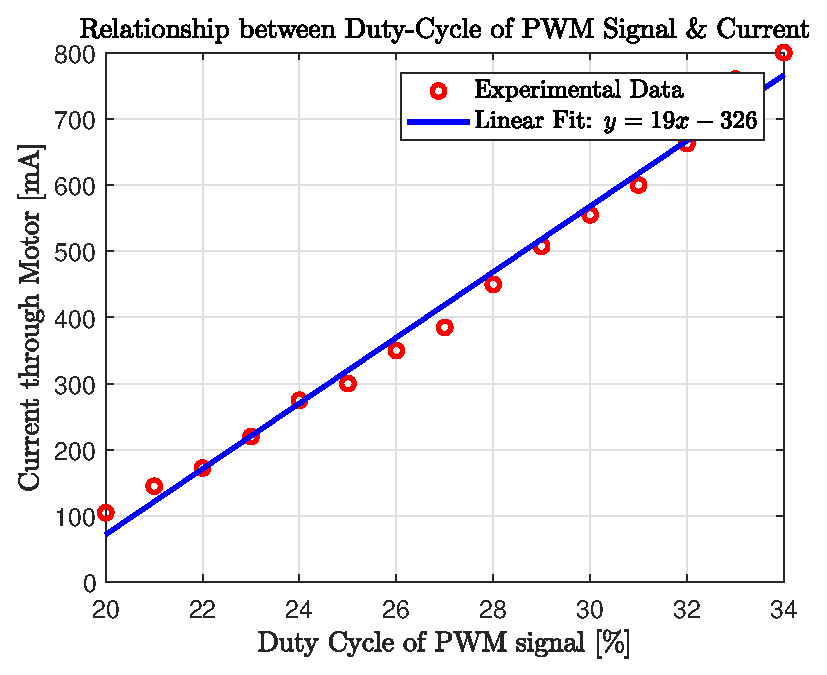
\includegraphics[scale=1]{./figs/dutycycle_vs_current.eps}
	\caption{Relationship between Duty-Cycle of PWM Signal and Current through Motor}
	\label{fig:dutycycle_vs_current}
\end{figure}

The input to the system is the torque delivered by the motor and the magnitude and direction is determined by the control laws. The model describing the system in equation \ref{eq:condense2} assumes the torque delivered to the system is instantaneously available. This is inaccurate due to the DC motor model describing the torque delivered by the model when applying a DC voltage. The input that the motor will be receiving is a Pulse-Width-Modulated (PWM) signal to represent a DC voltage.

Experiments were done to determine the relationship between the duty-cycle of the PWM signal and the torque delivered by the motor. These experiments are done by incrementing the duty-cycle of the PWM signal that the motor receives when the shaft is kept fix against a hard-stop. The motor-driver that controls the motor has a feedback pin that provides a proportional current of $\frac{1}{375}$ of the current flowing through the motor. This proportional current is allowed to flow through a known resistor. The voltage across the resistor is measured and provides a indication of the current flowing through the motor. The mean value of the voltage measured on the oscilloscope is taken and mapped backwards to determine the current. Figure \ref{fig:dutycycle_vs_current} shows the measured data with a line of best fit. It is clear that there exist a linear relationship between the duty-cycle of the PWM signal and the torque the motor can provide.